\documentclass{article}[18pt]
\usepackage{../../../../format}
\lhead{Software Engineering  - Project Management}


\begin{document}
\begin{center}
\underline{\huge Requirements Engineering II}
\end{center}
\section{Validation of requirements}
\begin{minipage}{0.8\textwidth}

Requirements Validation
\begin{itemize}
	\item Check that the \textbf{right product is being built}
	\item Ensures that the software being developed (or changed) will satisfy its stakeholders
	\item Checks the software requirements specification against stakeholders goals and requirements
\end{itemize}
Requirements verification:
\begin{itemize}
	\item Check that the \textbf{right product is being built right}
	\item Ensures that each step followed in the process of building the software yields the right products
	\item Checks consistency of the software requirements specification artefacts and other software development products (design, implementation, ...) against the specification
\end{itemize}
Requirements error costs are so high so validation is very important
\begin{itemize}
	\item Fixing a requirements error after delivery may cost up to 100 times the cost of fixing an implementation error
\end{itemize}

\end{minipage}
\begin{minipage}{0.2\textwidth}
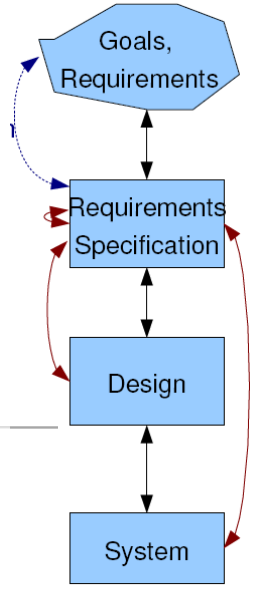
\includegraphics[scale=0.7]{validation}
\end{minipage}
Help ensure delivery of what the client wants\\
Need to be performed at every stage during the (requirements) process
\begin{itemize}
	\item Elicitation
	\begin{itemize}
		\item Checking back with the elicitation sources
		\item "So, are you saying that ...?"
	\end{itemize}
	\item Analysis
	\begin{itemize}
		\item Checking that the domain description and requirements are correct
	\end{itemize}
	\item Specification
	\begin{itemize}
		\item Checking that the defined system requirement will meet the user requirements under the assumptions of the domain/environment
		\item Checking conformity to well-formedness rules, standards ..
	\end{itemize}
\end{itemize}
\section{Requirements checking}
\begin{itemize}
	\item Validity checks - Does the system provide the functions which best support the customer's needs?
	\item Consistency checks - Are there any requirements conflicts?
	\item Completeness checks - Are all functions required by the customer included?
	\item Realism checks - Can the requirements be implemented given available budget and technology?
	\item Verifiability checks - Can the requirements be checked (tested)?
	\item Traceable - Where/who did the requirement come from and rationale?
\end{itemize}
\section{How to make the requirements testable}
Each requirement carries a \textbf{fit} criteria\\
The fit criteria are a benchmark, or goal, that the testing activity used to determine whether the eventual solution satisfies the requirement\\
\\
For FR - the function is either completed or not - no scales of measure\\
For NFR is a quality the product must have, fit criterion is a measure of that\\
\\
If such criteria cannot be easily expressed or quantified then the requirement is likely to be ambiguous, incomplete or incorrect\\
\\
Relatively easy of determine fit criteria for quality requirements that are naturally quantitative e.g. performance, size, accuracy 
\section{The system with assumptions}
\begin{itemize}
	\item Often the requirements for a system-to-be include assumptions about the environment of the system
	\item The system specification S, then, has the form
	$$S=A\Rightarrow G$$
	\begin{itemize}
	\item where A are the assumptions about the environment and G are the guarantees that the system will meet the requirements as long as A holds
	\end{itemize}
	\item If these assumptions (A) are implied by the known properties of the domain (D), that is $D\Rightarrow A$, and we can check that the domain properties (D) and the system guarantees (G) imply the requirements (R), that is D and G$\Rightarrow$ R, then the validation condition, D and S $\Rightarrow$ R is satisfied
\end{itemize}
\section{Formal Verification and Validation}
Evaluating the satisfaction of "D and S$\Rightarrow$ R" is difficult with natural language
\begin{itemize}
	\item Descriptions are verbose, informal, ambiguous, incomplete ...
	\item This represents a risk for the development and organization
\end{itemize}
Verification of this "validation question" is more effective with formal methods (see below)
\begin{itemize}
	\item Based on mathematically formal syntax and semantics
	\item Proving can be tool-supported
\end{itemize}
Depending on the modelling formalism used, different verification methods and tools may be applied. We call this "Model-Based V\& V"
\section{V\&V vs Analysis}
Both have several activities in common
\begin{itemize}
	\item Reading requirements, problem analysis, meetings and discussions ...
\end{itemize}
Analysis works with raw, incomplete requirements as elicited from the system stakeholders
\begin{itemize}
	\item Develop a software requirements specification document
	\item Emphasis on "we have the right requirements"
\end{itemize}
Requirements V\&V works with a software requirements specification and with negotiated and agreed (and presumably complete) domain requirements
\begin{itemize}
	\item Check that these specifications are accurate
	\item Emphasis on "we have the right requirements well done"
\end{itemize}
\section{Requirements V\&V Techniques}
Various types:
\begin{itemize}
	\item Simple checks  - traceability, well-written requirements
	\item Prototyping
	\item Functional test design
	\item User manual development
	\item Reviews and inspections
	\begin{itemize}
		\item Walkthroughs
		\item Formal inspections
		\item Checklists
	\end{itemize}
	\item Model-Based V\& V
	\begin{itemize}
		\item First order logic
		\item Behavioural models
	\end{itemize}
\end{itemize}
\subsection{Simple Checks}
Various checks can be done using traceability techniques
\begin{itemize}
	\item Given the requirements document, verify that all elicitation notes are covered
	\item Tracing between different levels of requirements
	\begin{itemize}
		\item Checking goals against tasks, features, requirements ...
	\end{itemize}
\end{itemize}
Involves developing a traceability matrix
\begin{itemize}
	\item Ensures that requirements have been taken into consideration (if not there should be a reason)
	\item Ensures that everything in the specification is justified
\end{itemize}
\subsection{Prototyping}
\begin{itemize}
	\item The prototyping process can start with those requirements which are poorly understood - helps stakeholder understand what the system will do
	\item Prototyping can be used to animate requirements (can build on earlier prototype)
	\item Prototypes for validation must be more complete than for elicitation - must contain sufficient facilities so practical used can be made of it
	\item Implementation of a number of features helps user identify important features and those not so important
	\item Useful for questions about user interfaces
\end{itemize}
\subsection{Functional Test design}
Functional tests at the system level must be developed sooner or later...
\begin{itemize}
	\item Can (and should) be derived from the requirements specification
	\item Each (functional) requirement should have an associated test
	\item Non-functional (e.g. reliability) or exclusive (e.g. define what should not happen) requirements are harder to validate with testing
	\item Each requirements test case must be traced to its requirements
	\item Inventing requirements tests is an effective validation techniques
\end{itemize}
Designing these tests may reveal errors in the specification (even before designing and building the system)
\begin{itemize}
	\item Missing or ambiguous information in the requirements description may make it difficult to formulate tests
\end{itemize}
Some software development processes (e.g. agile methods) begin with tests before programming test-driven development (TDD)
\subsection{User Manual Development}
Same reasoning as for functional test design:
\begin{itemize}
	\item Has to be done at some point
	\item Reveals problems earlier
\end{itemize}
Forces a detailed look at requirements\\
Particularly useful if the application is rich in user interfaces/for usability requirements\\
\\
Typical information in a user manual
\begin{itemize}
	\item Description of the functionality
	\item How to get out of trouble
	\item How to install and get started with the system
\end{itemize}
\subsection{Reviews and inspections}
A group of people (mix of stakeholders) read and analyse requirements, look for potential problems, meet to discuss the problems, and agree on a list of action items needed to address these problems\\
\\
A widely used requirements validation technique
\begin{itemize}
	\item Reading the document - a person other than the author of the document
	\item Reading and approval (sign off) - encourages the reader to be more careful (and responsible)
	\item Walkthroughs (informal)
	\item Inspections (formal) - very structured and detailed review, defined roles for participants, preparation is needed, exit conditions are defined
\end{itemize}
Can be expensive, requires careful planning and preparation
\begin{itemize}
	\item Need appropriate checklists (must be developed if necessary and maintained)
\end{itemize}
Advantages
\begin{itemize}
	\item Effective (even after considering cost)
	\item Allow finding sources of errors (not only symptoms)
	\item Requirements authors are more attentive when they know their work will be closely reviewed
	\item Familiarise large groups with the requirements (buy-in)
	\item Diffusion of knowledge
\end{itemize}
Risks
\begin{itemize}
	\item Reviews can be dull and draining (need to be limited in time)
	\item Time consuming and expensive (but usually cheaper than the alternative)
	\item Personality problems
	\item Office politics
\end{itemize}
\subsection{Model-based (formal) V\& V}
Available V\&V techniques will vary from one modelling paradigms to another and will also depend on the available tools\\
\\
The following functions may be provided through tools:
\begin{itemize}
	\item Completeness checking: only according to certain syntax rules, templates
	\item Consistency checking: given model M, show that M does not imply a contradiction  and does not have any other undesirable general property (e.g. deadlock possibility)
	\item Refinement checking: given two models M and M’, show that the properties of M imply the properties of M’. This can be used for the validation of the system specification S, that is, showing that  D and S $\Rightarrow$ R where D are the domain properties and R are the domain requirements (M = D and S; M’ = R)
	\item Model checking: given a model M and some properties P, show that any system implementation satisfying M will have the properties P
	\item Generation of system designs or prototype implementations (from workflow or state machine models)
	\item Generation of test cases 
	\item Performance evaluation
\end{itemize}
\section{The requirements document}
\begin{itemize}
	\item It is NOT a design document. As far as possible, it should set of what the system should do rather than how it should do it
	\item Give full visibility and secure record of the required behaviour
	\item Ensure correct information is accurately communicated to the developers, facilitates future maintenance
	\item Provide a baseline against which functionality can be tested
	\item Provide information for production of user manuals etc.
	\item To facilitate future development of new systems with similar functionality
	\item It’s an official statement of what the system developers should implement
\end{itemize}
\section{IEEE propose Requirements Documents to be..}
\begin{itemize}
	\item Unambiguous - requirements are often written in a natural language where statements can have more than one meaning. Formal requirements languages help reduce ambiguity because formal language processors automatically detect many lexical, syntactic and semantic errors
	\item Complete - The requirements document is complete if it includes all the significant requirements, whether relating to functionality, performance, design constraints, attributes or external interfaces and conforms to the company standard
	\item Verifiable - an example of a non-verifiable requirement ‘the product should have a good human interface’. An example of a verifiable requirement ‘the system will respond to a users request within 20 seconds of the user pressing the enter key, 80\% of the time.
	\item Consistent - these types of conflict can occur
	\begin{itemize}
		\item different terms used for the same object: for example, a ‘P45’ and a ‘tax form’ might be used to describe the same form
		\item characteristics of objects conflict: different parts of the document state different actions for dealing with faults
		\item Logical or temporal faults: for example, ‘A follows B’ and A and B occur simultaneously to another
	\end{itemize}
	\item Modifiable - the requirements document should have a coherent and easy-to-use organisation, with a table of contents, an index and explicit cross referencing. Statements should be non-redundant where possible
	\item Correct - every requirement listed within the document will be met by the software
	\item Traceable - the origin of each requirement should be clear, thus facilitating ‘backward traceability’ to previous decisions made and ‘forward traceability’ to all documents ‘spawned’ from the requirements
	\item Usable - The requirements document should be designed such that it can be referred to and if necessary modified throughout the life of the product. It should be usable even in the operation and maintenance phase
	\item Ranked - The requirements should be ranked by importance (for instance critical, important, desirable). Assessment to be made by developer/ users
\end{itemize}
\section{Guidelines for writing requirements}
Invent a standard format and use it for all requirements\\
Use language in a consistent way. Use shall for mandatory requirements, should be for desirable requirements\\
Use text highlighting to identify key parts of the requirements\\
Avoid the use of computer jargon\\
To ensure requirements are traceable they must have
\begin{itemize}
	\item A unique number
	\item An identifier of the type of requirement or constraint
	\item Reference to all of the business events and use cases that contain the requirement
	\item References to dependent requirements that might use the same matter, or have some change effect on this one
	\item Consistent use of terminology
\end{itemize}
\end{document}